%!TEX root = ./main.tex

%%**************************************************************
%%
%%	 DHBW Stuttgart Campus Horb
%%
%% 	Schwer vereinfachte Version einer generellen Vorlage 
%%	für Arbeiten an der DHBW
%%	Original-Vorlage erhältlich unter:
%%        https://github.com/schnes4/dhbw-heidenheim-latex-template
%%
%% 	Die Originalvorlage wurde von Studenten in Horb geschaffen
%% 	und von Studenten in Heidenheim später noch erweitert/angepasst
%%
%%**************************************************************


% show warning for old LaTeX syntax
\RequirePackage[l2tabu, orthodox]{nag}

% DOCUMENT CLASS Definition
\documentclass[
	pdftex,
	oneside,  
	12pt,			   	 % fontsize
	parskip=half,		 % Space (in lines) between paragraphs	
	headheight = 12pt,    	% Header hight
	headsepline,		    	% Line after header
	footheight = 16pt,	    	% Footer height
	footsepline,		   	 % Line before footer
	abstract=true,		% Abstract headline
	DIV=calc,		    	% Calculate print space
	BCOR=8mm,		    	% BCOR settings (Bindekorrektur)
	headinclude=false,   	% Exclude header from print space
	footinclude=false,	    	% Exclude footer from print space
	listof=totoc,		    	% Show List of Figures/Tables in Contents
	toc=bibliography,	    	% Show Bibliography in Contents
]{scrreprt}	                    		 % Koma-Script report-class, long document: scrreprt, short document: scrbook


% Prepare for utf and german
\usepackage{xstring}
\usepackage[utf8]{inputenc}
\usepackage[T1]{fontenc}

\usepackage[ngerman]{babel}


%% Fonts
%% palatino, goudysans, lmodern or libertine
\newcommand{\documentFont}{lmodern}

%% Margin
\newcommand{\margin}{2.5cm}

%% Space between chapter headline and top of page
\newcommand{\chapterMargin}{20pt}

%% Table settings
% Column spacing
\newcommand{\tableColumnMargin}{10pt}
%Line spacing
\newcommand{\tableRowMargin}{1.5}

%% Color settings
\newcommand{\defineColors}{%
	\definecolor{LinkColor}{HTML}{\linkColor}
	\definecolor{ListingBackground}{HTML}{F8F8F8}
}
\newcommand{\linkColor}{00007A}

%%% Definitionen für gute Code Listings
%%% DEFAULT Programmiersprache ist auf Java gesetzt (language=Java)
%%% entsprechend ändern wenn nötig
%% Syntax Highlighting (Listings)
\newcommand{\listingsettings}{%
	\lstset{%
		language=Java,			% default language
		numbers=left,			% position of line numbers (left, right)
		stepnumber=1,			% set number to each line
		numbersep=5pt,			% 5pt between number and source code
		numberstyle=\tiny,			% letter size of numbers
		breaklines=true,		       	 % break lines if necessary (true, false)
		breakautoindent=true,	        	% indenting after break line (true, false)
		postbreak=\space,			% break line after space
		tabsize=2,				% tabulator size
		basicstyle=\ttfamily\footnotesize, % font style
		showspaces=false,			% show space (true, false)
		extendedchars=true,		% show all Latin1 characters (true, false)
		captionpos=b,			% sets the caption-position to bottom
		backgroundcolor=\color{ListingBackground}, % source code background
		xleftmargin=10pt,		        % margin left
		xrightmargin=5pt,		        % margin right
		frame=single,			% border settings
		frameround=ffff,
		rulecolor=\color{darkgray},	% border color
		fillcolor=\color{ListingBackground},
		aboveskip=20pt,
		keywordstyle=\color[rgb]{0.133,0.133,0.6},
		commentstyle=\color[rgb]{0.133,0.545,0.133},
		stringstyle=\color[rgb]{0.627,0.126,0.941}
	}
}




\usepackage[margin=\margin,foot=1cm]{geometry}
\usepackage[activate]{microtype}                                         
\usepackage[onehalfspacing]{setspace}
\usepackage{makeidx}
\usepackage[autostyle=true,german=quotes]{csquotes}
\usepackage{longtable}
\usepackage{enumitem}	                                                 
\usepackage{graphicx}
\usepackage{pdfpages}                                                         
\usepackage{xcolor} 	                                                    
\usepackage{float}
\usepackage{array}
\usepackage{calc}		                         
\usepackage[right]{eurosym}
\usepackage{wrapfig}
\usepackage{pgffor}                                                             
\usepackage[perpage, hang, multiple, stable]{footmisc}  
\usepackage[printonlyused]{acronym}                                 
\usepackage{listings}
\usepackage[obeyFinal,backgroundcolor=yellow,linecolor=black]{todonotes}
\usepackage{rotating}
\usepackage{lscape}
\usepackage{amsmath}
\usepackage{amssymb}
\usepackage{\documentFont}

\usepackage{bookmark}
\usepackage[nonumberlist,toc]{glossaries}

% custom added
\usepackage{pgfplots}
\pgfplotsset{compat=1.18}

% Generate glossary
\makeglossaries{}

% Load colors
\defineColors{}

% Set Titel, Autor and Date
%\title{Titel der Arbeit}
%\author{Max Mustermann}
%\date{xx. Monat 202x}


\usepackage{caption} % finally correct hyperlinks
% PDF link settings
\hypersetup{%
	colorlinks=true, 		
	linkcolor=LinkColor, 	
	citecolor=LinkColor,
	filecolor=LinkColor,
	menucolor=LinkColor,
	urlcolor=LinkColor,
	linktocpage=true, 
	bookmarksnumbered=true 
}

% Captions fontsize
\addtokomafont{caption}{\small}




%% HIER wählen wir BIBLATEX
% Bibliographie settings

%% Richtige style zum zitieren
% http://ctan.mirrorcatalogs.com/macros/latex/contrib/biblatex/doc/biblatex.pdf (3.3.1 Citation Styles)
% recommended:  z.B numeric-comp, alphabetic, 
% not recommended: authoryear, alphabetic-verb, 
\newcommand{\quoteStyle}{alphabetic}

\usepackage[
	backend=biber,		% recommended. Alternative: bibtex
	bibwarn=true,
	bibencoding=utf8,	         % If .bib file is encoded with utf8, otherwise ascii
	sortlocale=de_DE,
	style=\quoteStyle,
]{biblatex}

\addbibresource{bibliographie.bib}  % die Bib-Latex Datei mit Ihrer Literatur


%% Put your images in the image directory
% Graphicspath
\graphicspath{{images/}}


% frequently used programing languages (to make perfect code listings)
\lstloadlanguages{PHP,Python,Java,C,C++,bash}

\listingsettings{}
% Rename Listings
\renewcommand\lstlistingname{Listing}
\renewcommand\lstlistlistingname{Listings}
\def\lstlistingautorefname{Listing}

% Spaces in tables
\setlength{\tabcolsep}{\tableColumnMargin}
\renewcommand{\arraystretch}{\tableRowMargin}





%!TEX root = ../main.tex

%
% To create glossary run the following command: 
% makeglossaries main.acn && makeglossaries main.glo
%

%
% Glossareintraege --> referenz, name, beschreibung
% Aufruf mit \gls{...}
%
 		% glossar-datei im Ordner content





%%%
%%% 	END OF THE DOCUMENT SETUP
%%%	DOCUMENT BEGINS HERE





\begin{document}

%% The Titlepage

\begin{spacing}{1}
\begin{titlepage}
	\begin{longtable}{p{8cm} p{8cm}}
		\raggedright {\raisebox{\ht\strutbox-\totalheight}{
\includegraphics[height=2.5cm]{images/cover/logo-dhbw.pdf}}} &
		% folgende Zeile nur einfügen bei Praxisarbeiten
		%\raggedleft {\raisebox{\ht\strutbox-\totalheight}{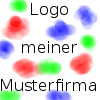
\includegraphics[height=2.5cm]{images/cover/logo-company.png}}}
	\end{longtable}
	\enlargethispage{20mm}
	\begin{center}
	\doublespacing{
		\vspace*{12mm}	{\LARGE\textbf {Entwicklung einer Schach-Trainingsanwendung zur Erlernung von Eröffnungen unter Verwendung von Schach-APIs}}\\
		\vspace*{12mm}	{\large\textbf {Studienarbeit (Modul T3\_3101)}}\\
		
		% Nur für die Bachelorarbeit (Sonst löschen)
	    %\vspace*{12mm}	für die Prüfung zum\\
		%\vspace*{3mm}	Bachelor of Science\\
		% End Bachelorarbeitsangabe

		\vspace*{12mm}	des Studiengangs Informatik\\
    		\vspace*{0mm}	an der DHBW Stuttgart Campus Horb\\
		\vspace*{12mm}	von\\
		\vspace*{3mm}	{\large\textbf Marvin Schlegel}\\
		\vspace*{12mm}	\today\\

	}
	\end{center}
	\vfill
	\begin{spacing}{1.2}
	\begin{tabbing}
		mmmmmmmmmmmmmmmmmmmmmmmmmm             \= \kill
		%\textbf{Bearbeitungszeitraum}       \>  12 Wochen\\
		\textbf{Matrikelnummer, Kurs} 	  \>  1490481, INF2022\\

		% Folgendes braucht man nur für die Praxisarbeiten:
		%\textbf{Ausbildungsfirma}               \>  Firmenname\\
		%\textbf{Ort}				\> Firmenort\\
		%\textbf{Betreuer}              	 \>  Firmenbetreuer\\
		% Folgendes braucht man nur für die Bachelorarbeit
		%\textbf{Zweitgutachter}		\>  Prof. Dr. phil. Antonius van Hoof\\

		% Bei Studienarbeiten / Seminararbeiten reicht:
		\textbf{Betreuer}              \>   Daniel Schaber\\
	\end{tabbing}
	\end{spacing}
\end{titlepage}
\end{spacing}

\newpage

\pagenumbering{Roman}

%% Die Erklärung: Bitte Titel der Arbeit Autor usw. noch anpassen!!

\thispagestyle{empty}

\section*{Ehrenwörtliche Erklärung}
\vspace*{2em}
Ich versichere hiermit, dass ich meine Arbeit mit dem Thema \emph{Entwicklung einer Schach-Trainingsanwendung zur Erlernung von Eröffnungen unter Verwendung von Schach-APIs} selbstständig verfasst und keine anderen
als die angegebenen Quellen und Hilfsmittel benutzt habe.

Ich versichere zudem, dass die eingereichte elektronische Fassung mit der gedruckten Fassung
übereinstimmt.

\vspace{3em}

ORT, DATUM

\vspace{4em}

\rule{6cm}{0.4pt}\\
AUTOR

\newpage

% Abstract
%!TEX root = ../main.tex

\pagestyle{empty}

% override abstract headline
\renewcommand{\abstractname}{Abstract}

\begin{abstract}
Im Rahmen dieser Arbeit wurde untersucht, wie Menschen lernen, mit dem Fokus auf Schacheröffnungen. Dabei stellte sich heraus, dass es besonders wichtig ist, Inhalte zu wiederholen.
Im Optimalfall sollten sie in exponentiell größeren Abständen wiederholt werden.
% Im Optimalfall werden sie in exponentiell größer werdenden Abständen wiederholt.
% Im Optimalfall wiederholt man sie mithilfe von Spaced Repetition in exponentiell größer werdenden Abständen.
Das aktuelle Angebot an Lernmedien, bietet diese Funktionalität aber selten. Daher wurde in dieser Arbeit eine Webseite erstellt, auf der Schachspieler Eröffnungen interaktiv betrachten und üben können. Den Nutzern wird zudem eine Empfehlung gegeben, welche Eröffnungen als Nächstes wiederholt werden soll, basierend auf den genannten wissenschaftlichen Erkenntnissen. Das entstandene Produkt lässt sich gut in Verbindung mit bestehenden Lernmedien verwenden.
\end{abstract}
		% Abstract in separate file in contents directory
\newpage

 % only page number in footer
\pagestyle{plain}
	
% space bevore chapter headline
\RedeclareSectionCommand[beforeskip=\chapterMargin]{chapter}

%%% Jetzt folgen die ganze Verzeichnisse

% Contents
\begin{spacing}{1.1}
\begingroup	
	% set subchapter depth
	\setcounter{tocdepth}{2}
	\tableofcontents
	\clearpage
\endgroup
\end{spacing}
\newpage

% Acronyms
\cleardoublepage
%!TEX root = ../main.tex

\addchap{Abk\"urzungsverzeichnis}

\begin{acronym}[YTMMM]

\acro{MCTS}{Monte Carlo Tree Search}
\acro{UCI}{Universal Chess Interface}
\acro{API}{Application Programming Interface}
\acro{REST}{REpresentational State Transfer}
\acro{TCEC}{Top Chess Engine Championship}
\acro{NNUE}{Efficiently Updatable Neural Network}
\acro{PGN}{Portable Game Notation}
\acro{CCRL}{Computer Chess Rating Lists}
\acro{URI}{Unique Resource Identifier}
\acro{MVC}{Model View Controller}
\acro{ORM}{Object Relational Mapping}
\acro{MAC}{Message Authentication Code}
\acro{HMAC}{Hash-based MAC}
\acro{JWT}{JSON Web Tokens}

\end{acronym}


% List of Figures
\cleardoublepage
\listoffigures

%List of Tables
\cleardoublepage
\listoftables

% List of Listings
\cleardoublepage
\lstlistoflistings
\cleardoublepage

\pagenumbering{arabic}
	
\pagestyle{headings}


%%% AB HIER KOMMEN DIE KAPITEL (.tex Dateien im content-Verzeichnis)

%Content
\foreach \i in {01,02,03,04,05,06,07,08,09,...,99} {%
	\edef\FileName{content/chapter/\i .tex}%
		\IfFileExists{\FileName}{%
			\input{\FileName}
		}
		{%
			% No chapter available
		}
	}

\clearpage

%%% AB HIER DANN LITERATUR, GLOSSAR und evtl. ANHANG

\pagestyle{plain}

% Bibilography
\cleardoublepage
\printbibliography

% Glossar
% \cleardoublepage
% \printglossary[style=altlist,title=\glossaryPhrase]
%%!TEX root = ../main.tex

%
% To create glossary run the following command: 
% makeglossaries main.acn && makeglossaries main.glo
%

%
% Glossareintraege --> referenz, name, beschreibung
% Aufruf mit \gls{...}
%

	
% Appendix
% \clearpage
% \appendix
%% !TeX root = ../main.tex

\addchap{Anhang}

Hier ist etwas f\"ur den Anhang.


	
\end{document}


